\subsection{Relay Scheme}
\subsubsection{BTC-Relay}
\noindent In 2016, the BTC-Relay released by the Consensys team is the most classic relay cross-chain solution, enabling cross-chain transactions between Ethereum and Bitcoin, as well as realizing Ethereum's DApp applications to support BTC payments. Since Bitcoin scripts are non-Turing complete and difficult to support complex applications, BTC-Relay only implements one-way cross-chain from Bitcoin to Ethereum.
        \begin{figure}[H]
        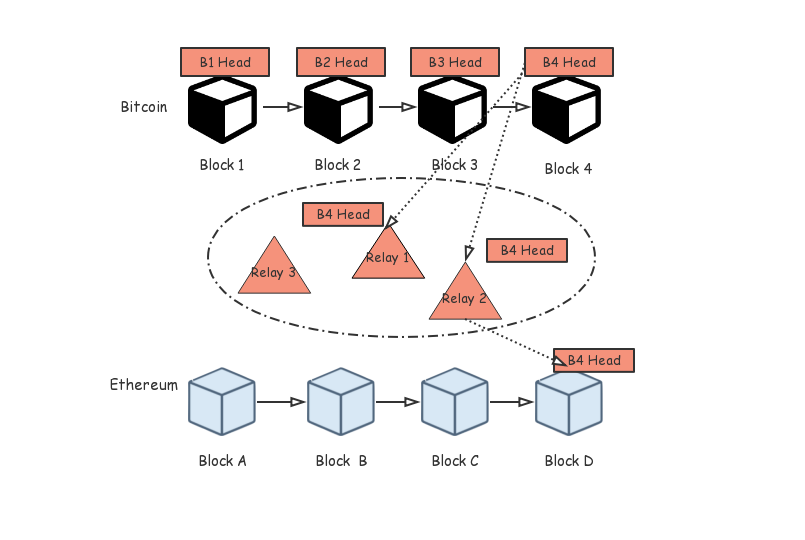
\includegraphics[width=1\textwidth]{./figures/btc.png}
        \centering
        \caption{BTC-Relay cross-chain process diagram}%\protect\footnotemark}
        \centering
        \label{fig:btc}
        \end{figure}
\noindent Like Figure \ref{fig:btc} shows, BTC-relay itself is a smart contract for Ethereum. The function of the contract is to verify certain transactions on Bitcoin and provide verification information to other DApp users on the Ethereum. Relay is a group of users who obtain block header data from Bitcoin and has the account address of the Ethereum network. The Relay that submits the block header data to the BTC-Relay contract as soon as possible can get the ETF transaction fee reward. After obtaining the block header data, the BTC-Relay smart contract can verify a transaction according to the principle of SPV proof. When a transaction in the Bitcoin network does occur, it can trigger the specific transaction or smart contract execution of the Ethereum network.

\subsubsection{Cosmos}
\noindent Cosmos\cite{cosmos} is a cross-chain platform project initiated by the Tendermint team in 2017. It supports the modular establishment of Cosmos isomorphism chain and also supports the external heterogeneous chain through Bridge. Its most important feature is that all the chains in the Cosmos system are isomorphic and can more easily support the flow of assets across the chain. All the zones share a set of network protocols, consensus mechanisms, and data storage methods. Assemble the new Zone blockchain through the API interface.\\
\noindent The overall architecture of Cosmos network are shown in Figure\ref{fig:cosmos}:

        \begin{figure}[H]
        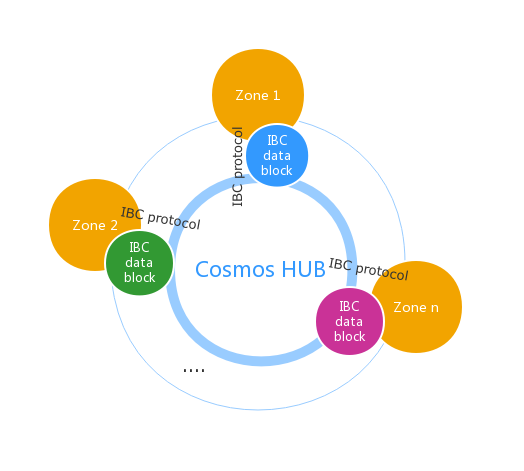
\includegraphics[width=0.8\textwidth, height=2in]{./figures/cosmos.png}
        \centering
        \caption{Cosmos network architecture\protect\footnotemark[1]}
        \centering
        \label{fig:cosmos}
        \end{figure}
  \footnotetext[1]{Figure taken from: \url{https://golden.com/wiki/Cosmos_network}}
        
\noindent There are many Zones connected to the Hub (Hub is a chain, and each Zone is also a chain). Cosmos Hub maintains a multi-asset distributed ledger and masters the asset status of all the Zones that connected to it. Each Zone will synchronize the state of the Hub, but the communication among Zones can only be done indirectly through the Hub. Each cross-chain asset transfer requires a standard successful confirmation from Zones and Hub. \\
\noindent The information is transmitted between zones through packets based on the IBC (Inter-Blockchain Communication) protocol. The blocks in a space pack the data to be delivered into standard IBC data packets and finally complete the transmission through the network layer UDP or TCP protocol.
        \begin{figure}[H]
        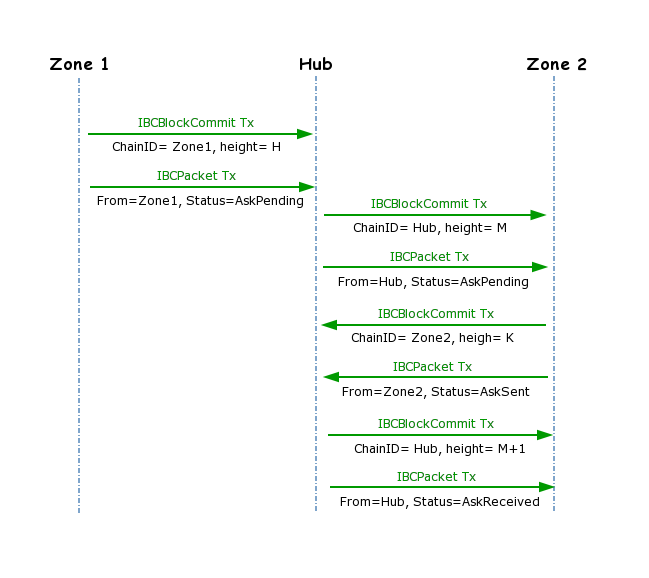
\includegraphics[width=0.8\textwidth]{./figures/IBC.png}
        \centering
        \caption{IBC sequence diagram}%\protect\footnotemark}
        \centering
        \label{fig:IBC}
        \end{figure}
\begin{enumerate}
    \item  Zone 1 initiates an IBCBlockCommitTx transaction, passing the new block header information (including all Validator's public key) to the Hub;
    \item  Zone 1 initiates an assets transaction;
    \item Zone 1 verifies the transaction;
    \item Send the valid transaction into the message queue for Hub;
    \item Zone 1 listens to a new message in the queue, which generates Merkle proof, and sent to Hub as IBCPacketTx's Payload. (In each space there is an independent third-party relay program that produces Merkle Proof from the original chain and assembles it into a Packet and initiates the transaction, passing it to the receiving chain);
    \item Hub verifies that Merkle Proof is valid, if it is valid, send a message to Zone2 (The process of sending a message to Zone2 by Hub is the same as steps 1~6);
    \item Zone2 verifies that Zone1 is a valid transaction after receiving the Hub message. Send a message to Hub confirming that it can acquire assets from Zone1;
    \item The Hub sends a message to Zone2, sends the asset to Zone 2, and the asset transaction is completed.
\noindent Due to an attack or network error during the transfer process, it is possible for the message sent by Zone 2 to the Hub is lost, as shown in the figure\ref{fig:timeout} below, after waiting for a period of time, the Hub sends a message telling Zone1 that the current transaction is timeout and the transaction fails.
\end{enumerate}
        \begin{figure}[H]
        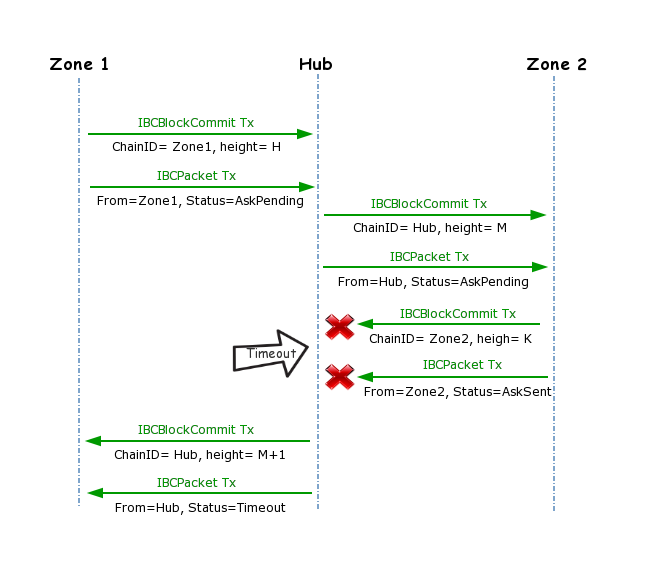
\includegraphics[width=1\textwidth]{./figures/IBC_timeout.png}
        \centering
        \caption{IBC sequence diagram, timeout}%\protect\footnotemark}
        \centering
        \label{fig:timeout}
        \end{figure}
        
\noindent Cosmos based on \textbf{Tendermint} consensus, which is the combination of PBFT and PoS, it improves the processing power of Cosmos Network. The cross-chain transaction between Cosmos and other heterogeneous blockchains need to be carried out through Cosmos Bridge, Bridge-Zone will be responsible for the docking with the original chain, including the confirmation of the original chain transaction, create or destroy the corresponding tokens.\\
\noindent Overall, Cosmos is a blockchain development framework, allowing developers to focus on their own business without having to consider the underlying technology of the blockchain so the plug-in design can use Cosmos as needed.

%
%\subsubsection{Polkadot}
%\noindent Polkadot\cite{polkadot} is a cross-chain project supported by the Web3 Foundation. Creating a scalable, heterogeneous, multi-chain architecture designed to address blockchain interoperability, scalability, and security.\\
%\noindent The overall architecture of Polkadot is shown in the figure below, consisting of a Relay Chain, Parachains and Bridges. \\
%
%\begin{table}[H]
%\begin{tabular}{l|c}
%
%Role& Description \\
%\hline
%\multirow{3}{1in}{\textbf{Relay chain}}& The central system of the Polkadot network, which \\& coordinates the consensus and transactions between the chains, \\& records account information and transaction status; \\
%\hline
%\multirow{2}{1in}{\textbf{Parachains}}& Built by developers to collect and process transactions,\\&and transfer to Relay chain; \\
%\hline
%\multirow{2}{1in}{\textbf{Bridges}} & Connects other heterogeneous blockchains (such as Ethereum) \\& with Polkadot network.\\
%\hline
%\textbf{Collators} & Collects user transactions and submitting to Validators\\
%\hline
%\multirow{2}{1in}{\textbf{Validators}} &Validates and broadcasts transaction data committed\\ & by Collators, verifys blocks and paying deposits\\
%\hline
%\textbf{Nominators} &Investment deposits selected for trust Validators \\
%\hline
%\textbf{Fishermen} &Supervises the evil behavior in the network\\
%\hline
%\end{tabular}
%\caption{Main roles in Polkadot}
%\end{table}
%
%\noindent Collators and Validators are the performers of the main transaction when doing cross-chain operations, while Nominators and Fishermen are the participants in maintaining system trust.\\
%
%
%\begin{figure}[H]
%    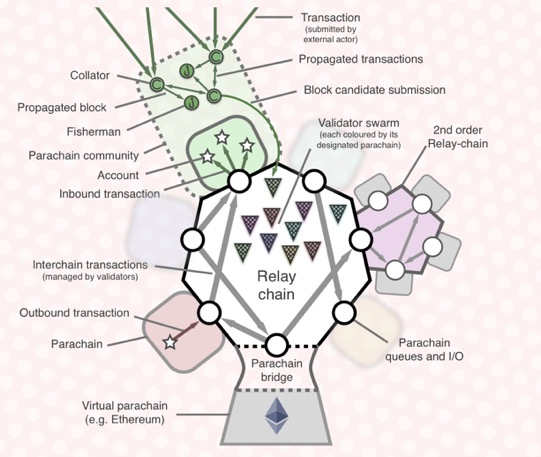
\includegraphics[width=1\textwidth]{./figures/Polkadot.jpg}
%    \centering
%    \caption{Polkadot network architecture \protect\footnotemark}
%    \centering
%\end{figure}
%\footnotetext{Image courtesy of Polkadot white paper\cite{polkadot}}
%
%\noindent Parachain can share trust of the entire Polkadot network, but it also gives a certain confirmation right to the Relay chain; when the user's transaction information on Parachain A is transmitted to Parachain B, the process is as follows:
%\begin{enumerate}
%    \item The initiated transaction is sent to the Collator on Parachain A;
%    \item Collator validates the transaction and packs it into the block; 
%    \item Collator submits the block and state transition proof to the Validator on Parachain A;
%    \item The Validator verifies the block it receives that contains only valid transactions and pays a certain amount of deposit;
%    \item  After enough Nominators have paid a deposit for the Validator, and they broadcast the block to the Relay Chain;
%    \item The transaction of data has been executed.
%\end{enumerate}
%\noindent Unlike Cosmos, Polkadot supports cross-chain interoperability between heterogeneous chains. It does support not only asset transactions but also data transfer. Its system complexity and implementation are more difficult than Cosmos.

%
%\subsubsection{Quant Overledger}
%\noindent Developed by Quant Network, Overledger is the one Blockchain Operating System that facilitates the development of multi-chain smart contracts\cite{verdian2018quant}. In order not to limit the inter-communication between 2 blockchains at the same time, Overledger enables reading the transactional, contract and script information and map them into one ``over layer''. So in most cases where the transaction requires multiple hops during the route to the destination, Overledger will create a common interface among ledgers to solve this issue.\\
%\noindent Different from other projects who devote their cross-chain solution into the transactional layer,





